\documentclass{standalone}
\usepackage{tikz}

\begin{document}
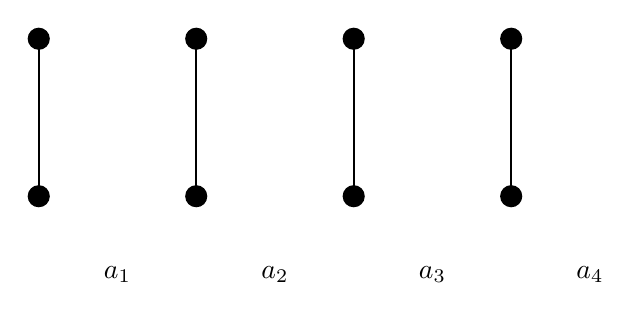
\begin{tikzpicture}[scale=2]
    % Define the points
    \foreach \i in {0,...,3} {
        \node (A\i) at (\i,0) {};
        \node (B\i) at (\i,1) {};
    }
    
    % Draw the arcs
    \draw[thick] (A0) -- (B0);
    \draw[thick] (A1) -- (B1);
    \draw[thick] (A2) -- (B2);
    \draw[thick] (A3) -- (B3);
    
    % Draw the crossings
    \fill (A0) circle (2pt);
    \fill (B0) circle (2pt);
    \fill (A1) circle (2pt);
    \fill (B1) circle (2pt);
    \fill (A2) circle (2pt);
    \fill (B2) circle (2pt);
    \fill (A3) circle (2pt);
    \fill (B3) circle (2pt);
    
    % Label the crossings
    \node at (0.5,-0.5) {$a_1$};
    \node at (1.5,-0.5) {$a_2$};
    \node at (2.5,-0.5) {$a_3$};
    \node at (3.5,-0.5) {$a_4$};
\end{tikzpicture}
\end{document}